\chapter{Thesis Project: Notebooks from Trashed Papers}


%****************************************
% Structure of Chapter:
% 
% Artist Statement
% Work
%  - Development of it.
%  - Parts of it. (Collecting, Transforming, Spreading them)
% Exhibition
%........................................


%****************************************
% Relationship between my project and theoretical aspects:
% - First one is actually is to analyze what is trash? Because I am using trash material and what is point of view of scholars to the trash. Realizing the potentials of it. Also the difference comes from the working on virgin object and trash object. Understanding the difference between the bricolouer and engineer. If trash has multiple life than these research will somehow reveal it. It is actually research on trash but what purposes. I guess it is missing? I need to set a purpose for the theory chapter. Or it is a just a background chapter? 
% - Roots in the art history. (Also roots on the social life can be researched?)
% - Inspiration from the other artist and also 
%........................................


%****************************************
% Sample Phrases
% \ldots is the concern of this study which aims to \ldots
% The aim is not to practice Antiquarian Avant-Garde techniques as a puritan form of photography, but rather to envision new means of photography.
% The aim of the thesis paper is to historically, socially and theoretically contextualize a student's work. The written thesis documents and informs the development and resolution of each student's artistic practice during the MFA program.
%........................................


% FROM Wild Art. quote taken from the television series `American Masters', Season 5, Episode 8, John Cage: I have nothing to say and I am saying it (aired on 17 September 1990).
\epigraph{The first question I ask myself when something doesn't seem to be beautiful is why do I think it's not beautiful? And very shortly you discover that there is no reason. If we can conquer that dislike, or begin to like what we did dislike, then the world is more open. That path ---of increasing one's enjoyment of life--- is the path, I think, we all best take: to use art not as self-expression, but as self-alteration; to become more open.}{\hfill---John Cage, \textit{Wild Art}}


In this chapter the artwork(thesis project) will be explained in detail. Final work and it's progress will be explained. Connection will be established with the previous chapters. Stages of work and concerns will be explained. 
%(Also the result of project is explained. But is there any result? I don't think so? I did not see discussions about the results of the works. but I try to collect peoples reflection and comments on it. Because I believe that it is not transforming the object.)

% What I have write is here to cover the project can not be sufficient. Because it is not possible to say everything about this project. I wish that this work would allow different interpretation and readings. 


% TODO
% Felix Gonzales Torres'in untitled işi benim yapmaya çalıştığım ile ilgili.


%%%
%%%
%%% 
% TODO
\section{Artist Statement}
(Collect, Save, Transform, Spread.)(Rescue, Revive)

% Converting disposal things to multiple time usage. Realizing the alternative lives of trash beyond their defined one shot life. Giving attention to the things. 

% Eğer bir artistic actten bahsediyorsak sadece bunun ürünle değil, üretimi ve insanların dahil olmasıyla desteklenebilir. Zaten toplama sürecinde bunu insanlarla ilişki kurarak yapıyorum. O insanlarda diğerleriyle konuşarak yapıyorlar.

% At this stage it is claimed that the process of transformation of trash can be treated as artistic act. In the production of notebooks people collected papers from different places and location. During the collection phase they also collect them from other people. In other words there is human communication during this process.

Actually (It is questioned that) working with trash dictates a life practice and, it is a convergence of behavioral patterns (attitudes toward to trash) and art making. The process effects one's life and lifestyle. (But what type of interaction between life and art making process?) (This claim is the main driving force of my artwork which is part of a thesis.) The purpose is not to build a thing that is produced from discarded material to watch it from a distance. The important thing is to interact with it. Because it is already discarded (disgusting, abject, unattractive etc.) and general behavior avoid from it, this work must change it. It must call the viewer to interact with it.

% Ersan hoca uzak seyretmek yerine etkileşime geçilmesini auranın kırılması olarak bakıyor. Performatif olması veya bir act olması zaten bunu kıran bir şey olabilir. Sanatsal eylem, performans kavramlarını araştırmak gerekli. Uzaktan seyredip hayranlık duymak yerine ilişkiye geçilen bir hale getirmek çöpü. Amaç bu aslında. Çöpü tekrar tanımak, onunla barışmak, onunla yaşamak. İşte bu yüzden bir eylem olabilir. Ya da yaşam pratiği. 

% Olay sadece böyle çöpten bir şeyler yapıp insanların seyretmesi değil, mühim olan onunla iletişime, ilişkeye geçmek. Yani zaten uzak durulan bir şey, onlardan bir şey üretildiğinde izleyici gene uzağında duruyorsa ne anlamı kaldı ki? İnsanların bu işin aşamalarının bir parçası olmalılar.

With the help of art (and artistic practices) discarded things can find a place in the society. (By the help of artistic approach things can be gain new values and meaning even if they are discarded and excluded from daily life (or society). The relationship between value creation and artistic practice examined through the artworks that uses trash as medium.)

% Using trash can not only understand in ecological perceptions, it also have powerful political claims. Or it should be examined in deeper levels beyond collage and assemblage, the medium itself has different meanings. 

% SEEING IT AS A RESOURCE.
Junk(or trash) can be seen as a new resource that is fertile to new meanings, creations and aesthetics. Ignored and discarded nature of garbage when rethought becomes fertile resource. Trash as a resource (as an artistic material). (City as a resource. Seeing the discarded items as a resource. Many artist approach to trash as resource. It is a shared approach. Some of them collect city discard, some of them tea cups, tea bags, discarded papers.)

% Çöpü tekrar ele alıp bir şeyler üretmek, onu tekrar yaşamımıza sokmak yeni alternatifler sunacaktır.

Do she/he want to take back (or revisit) the trash once thrown away? People do not want to think of what they throw away. Turning them to a things that worth to look again. How do artists reflect garbage and what are their tactics? What is the thing that add value to trash and what is the role of art in that?

With the help of art discarded things ---in the scope of thesis in particular paper trash--- can be transformed beyond the other industrial (or technological) methods. In other words autistics practices generates applies different methods.


%%%
%%%
%%%
\section{Inspired Works}
There are some works that inspire me a lot when developing the work. They are not actually trash related works therefore I put them in different section and here before the details of my work. However the previous chapter has also very inspirational contributions to the my work. They helped the understand the topic and develop an approach to the topic. In this section some projects are mentioned and their methodologies are explained. How are these works effected my work. What is the relationship between them? (Maybe all of them can be explained only the related part of it.)
\begin{itemize}
\item SketchBook Project. Inspires me a lot. Lots of works from all over the world. Full of creativity and showcase of richness of people's expressions on the small notebooks. My work can be considered as a sketch book project through trash. Sketches or only creative progress is not the only consideration. You can send your lecture notes. 
\end{itemize}


%%%
%%%
%%%
\section{Progress}
Here stages(progress) of my artwork are listed:

\begin{itemize}
\item \textbf{Memories.} As far as I know I collect things it is hard to say collecting started after an exact event or time but there are several memories that I remember. One of these (First of them) is from my primary school teacher. When I was third class my teacher give us a homework to bring colorful paper to make something(whatever it is I don't remember). The day after we bring some colorful paper but she did not. Instead of this she bring paper cut out from packages that are colorful, shinny and qualify. And I remember clearly that she suggest that same for us. Do not throw out packages, look for the useful parts and keep them to use later. 
\item \textbf{Motivation.} I can not throw them away. When I throw them I became sad for them. I have to find something useful for it. Even if I can not find it, I can pass it to another person who can make use of it for own purposes. We are humans that can produce, transform items. One of most developed species in the earth that produce and use tools. There is a lot of effort to produce thrown away and it seems that all this efforts are wasted. What I mention is not related about ultimate productivity. It is more close to being thoughtful, and taking responsibility of tools, items and objects that we are using. Rather than throwing out, creating a way that all are have chance to live together is much more close to my perception. 
\item \textbf{Collecting.} One of the most found trash in my habitat is paper. I work at METU Technopolis, live at 100. yil which is the nearest settlement to METU and study at Bilkent. People live there commonly use paper and needs paper. Paper is nearly everywhere. Reusing the paper is not limited with recycling of it. There is a another ways of it. When we recycle them actually we again send away them and use it as we all know. (industrial papers and notebooks.) There is no richness here. Same type of paper. Produced after a industrial process. I collected them from my friends (people that have communicate often). Sometimes I collect them from trash bins and roads. 
\item \textbf{Transforming.} I turned them to notebooks. Actually I use it for my self. And while I was using of it I am very proud of it. I am studying nearly more 20 twenty years and I have always need for notebooks and use them. It is some sort of passion for me notebooks. Because I always admire notebook beautifully design or uniquely designed. I collect them whenever I find and most of the time I only save them for later use. 
\end{itemize}

%%
%%
\subsection{Problems}
There are a lot of questions and problems that I have to overcome while development of my work. 

% Yani aslında bir derdim ve yapmak istediğim bir şey var. Ama bunu gerçekleştirmek için yapmam gereken şeyler var. Ve bunların bazılarının nasıl yapılacağı çok belli değil. Ben bunlara bir çözüm buluyorum. Bir yöntem üretiyorum. Bu kısımda aslında bunlardan bahsediyorum.

\begin{itemize}
\item First one is that my art work can be considered as design and has functional purposes. (It is not just a design, it is uses design to reach its goal like many artworks use other disciplines to reach their goals and expression. Purpose is not design and functionality.)
\item Using unused industrial paper. (Mixed trash and virgin material, \textbf{to show that discarded and desired object can live together.})
\item Collecting them with help of people, and asking other people to give the unused papers. (Collected from my close friends, from supervisor, from office where I work, from modshifters and varuna gezgin and from bcc labs(hopefully)?)
\item Giving them to people, but people should take them voluntarily.
\end{itemize}

%
\subsubsection{Functionality and Art Debate}
From an art historical perspective, you could say that functional art is the inverse of Marcel Duchamp's famous readymades, where he transformed utilitarian objects---a urinal, a bottle rack, etc.---into conceptual artworks by fiat: it became art because he said it was. Duchamp's works kills the functionality. It works beyond the functional perception. Moves the debate to the conceptual frame. However it is not every time case. Today many functional art objects are as avidly acquired by collectors as their fine-art brethren, and are appreciated just as much for their beauty as their use value. Ancient Chinese vases, for example, while still capable of performing their originally intended function (displaying flowers), are prized for their historic and aesthetic value more than anything else. \quotes{In conceptual art,} Sol LeWitt writes, \quotes{the idea or concept is the most important aspect of the work\ldots The idea becomes the machine that makes the art} \cite{lewitt1967paragraphs}. Therefore anything can be turned to art with a good idea. 

% TODO PRAP.
Comparing art to craft is like comparing philosophy to engineering: they're two separate ways of looking at the same thing. To me art is communication of an idea or an emotion, while craft is the physical manipulation of material. An object can easily be both, either, or neither. A sculpture, for example, may communicate, but it was constructed using craft. Likewise a teapot can communicate an idea, but it was crafted. Function is misleading and no distinction. Functional objects can still communicate ideas, so art can be functional. One object could be viewed two ways: if you look at the way it was made and the materials used, you are looking at its craft, if you think about its ideas, you are viewing it as art. An object could have been crafted, but contain no art. Even a painting can be crafted but artless. A ready-made might be art with no craft. I very much like the idea of a spectrum. One last thought: skill doesn't enter into the definition of art, since a piece could succeed as art but be poorly crafted.

\textbf{Why is it not a design?} Because the considerations and priorities are different? Functionality is not my primary concern. I do not increase the functionality or searching best functionality? (Considerations of design and art can be compared and what are my priorities in this work. I'm not trying to finish the garbage problem. Is it a problem for me? Do I problematize it?) 

\textbf{Why is it art?} Uses artistic methods? Does it represent anything? The idea is transforming things. Anything can be transformed and re-contextualized again. The limitation is our imagination and approach. It has a claim. In can be analyzed and examined in the context of art. It is hard to say that something is art or not. However it can be examined in the context of art. There are artworks reject art galleries. There are artworks also reject commodities. It has purpose that. spread out the idea in different manner. Subverts peoples ideas. 

The work aims to liberate the imagination and change the way people see the trash.

%%
%%
\subsection{Paper}
"Paper is an indispensable product throughout the world. Its primary use is as a medium for writing, essential for bureaucracy, education, communications, information storage, and in the spread of information. In addition, it is used for the packaging for transport and convenience of a wide range of items from food to industrial equipment. Paper also has specific technological uses, such as for filters and in art, home furnishings, and architecture, and it has a range of uses for hygiene purposes. Paper in several forms is consumed on a daily basis by each person in the Western world." \cite{trafford2012paper}

%
\subsubsection{Environmental Impact}
Paper is both biodegradable and a renewable resource, which means in consumption and waste terms, its environmental impact is relatively small compared to the many more-toxic and bulky waste products that are found in everyday garbage. However, the chemicals, water, and electricity used in its manufacture are considerable---and these are nonrenewable resources---and certain types of chemicals used in paper production are toxic. In addition, if waste paper is sent to a landfill, it releases carbon dioxide emissions. Further, forest resources are not always as renewable as one may like to think. These environmental impacts can be greatly reduced by recycling (paper being one of the most easily and cheaply recyclable products in everyday use) and by conscientious consumption practices.

Paper made exclusively from wood is called virgin paper, while paper produced out of used paper that is re-pulped is called recycled paper. Recycling paper can greatly diminish demand for virgin fiber from wood. However, there will always be a demand for virgin paper because, although paper is thought of as a renewable resource, it cannot be recycled indefinitely. It can only be recycled four to six times, as the fibers get shorter and weaker each time. In addition, some virgin pulp must be introduced into the process each time to maintain the strength and quality of the fiber, so no matter how much is recycled, paper will always need some virgin fiber.

% History of Paper
The word paper comes from papyrus, the plant that was first used for making a medium for writing in ancient Egypt.

% Production of Paper
All types and qualities of paper share the same basic method of manufacture, including newspaper paper, print paper, and carton used for boxes.

% Uses of Paper
Paper has become the most ubiquitous product in the age of information. Such products often complete their journey from shop floor to garbage in a single day; for example, newspapers, print paper, packaging, lavatory paper, tea bags, transport tickets, price tags, shopping bags, flyers, leaflets, wrapping paper, napkins, and tissues. 

%%
%%
\subsection{Why (package) paper?}
Easy to collect. Easy to find. Thrown out even if it is good quality. Packaging materials are very widespread. Appropriate for painting and writing. Has a very short life time. Disposable, there are a lot of package outside. No need to carry it. Every place gives you package paper. 

%%
%%
\subsection{Why covering notebooks and books?}
They are all package paper, already used as carry things and this work it has used again for the same purpose (but in different connection, this time trash is bound to the notebook). Trash is used to cover the papers. Cover is the most visible part of the notebook and book. Therefore trash becomes most visible part of the produced item. What is the function of cover? It gives ideas about what is inside, distinguishes from other things, protect it.

%%
%%
\subsection{Why giving away?}
Aim is to spread the idea by making something useful from trash. Increase diversity, activate (or encourage) people to embrace the trash.

%%
%%
\subsection{Why in the public space?}
To reach more audience. Actually the audience is out of the art galleries. They are walking in the streets. Putting them to next to people is much more effective. It is not visible and nearly it is hided from society. It is dirty. Removed from the society. There is a effort to hide them away. However in this project it is again showed to the society. Because it is revisited and reclaimed. 


%%
%%
\subsection{Artistic tactics}
Here I followed some tactics to realize my purposes. I called them artistic tactics. Easy to carry while traveling. Small notebooks. Placing them to their routes. 

\subsection{How I reached to notebook?}
Actually I have been collecting same materials that are used in my project before the thesis work. In my mind there is always belief that I can I find something useful for them. (In that time my main evaluation was to create useful object for my need.) Later it turned to an artwork. Before the thesis I also produce the notebooks for myself. However what is changed in thesis. First my approach to the trash is a little bit deeper. What is added to the notebooks. I started to use also used papers. for the cover of the notebook, I use more different materials. more close to collage. production method changed. and I started to collect different things, from different places. My realization increased. I organized my close friends and others to collect or save their trash for me. I discovered some points. their differences. 

% What I tried during this progress: Wrap out the trees, because I think that most of the materials that I collected are package papers. Well I somehow package the trees again. not to carry them but to raise awareness. Yani benim amacımı en iyi anlatacak olan şey nedir? Aslında ben burada defterden gidip bunu anlamlandırmaya çalıştım. Dolayısıyla deneyerek deftere nasıl ulaştım da ziyade defterden başlayıp nasıl tekrar defterde karar kıldığımı anlatan bir hikaye olabilir? Yani bu çok da şart olmayabilir bir diğer yandan da? Developlement of work? Nasıldı nereye geldi? How my project evolved? And this also explains how it is relates with the research. Because the reasearch is shaped the project also. Which part of the project shaped by the project? Not thinking in the ecological perspective. Raised questions also mature the project? For example zizek suggest that to find spirutuality and aesthetics to the trash, and for me? 

\textbf{Why notebook?} Because I already do it. So What I didn't change it. It is the best one or no to change it. I love idea of carrying notebook with near of you. I have also save my notebooks. I don't throw away them. A notebook is actually is a work of you. It carries your signature. It is one of best gift to give someone. Because it is a combination of your work and the other peoples works. It is co-authored work. Actually there is also a part of people who throw away this peace. Actually the best part of it the transformation is not finishes after my creation of notebook. It continues with the usage of it. How it turned to is not actually uncertain. Therefore it is very appropriate of my idea that transforming trash is increases the diversity.

\textbf{What is different from industrial notebooks?} Handmade, from trash. an alternative to other versions. every one have different stories, they are different in visuals (but the others are also different.) What makes them different is not clear actually. Does it have to be different? Yes. The production method is different. You pay no money. There is different with gift notebooks from companies. This notebooks call to you change the destiny of trash together. 

\subsection{What do I think about trash?}
I need to clarify my approach to the trash, wasting and discarding. First point is that I am very uncomfortable to the action of discarding thing. I always think that by discarding this think I am missing something rather than getting rid of something. Sometimes because of the significant amount of residue from consumption from daily activities I became overwhelmed and to move on I need to leave behind them and move on. However almost it is never ending loop. (I believe that sometimes we need to break the loops to realize different meanings. To think outside the box, we need to behave outside of common habits. As I mentioned the discarding things are some of the loops that we are rare to behave like other way.) \textbf{What am I discarding?} To get rid of my load and move on. But for what? and also ought to be like that? (throw away them to same bin. (Some of people do not care too much bin and throw them whenever it is possible.)) Even if I discard some stuff I think that I am ignoring its potential and losing it. At that times I become very sad and feel very comfortable. I must have find to another place for it more suitable than a waste bin. At least I can give them someone else who can use it for own purposes. Do I really luxury of discard?

Significance of thinking outside the box (about actually trash) is actually breaking the loops. You have to look at differently from your common perception. \textbf{Break the rules, break the loops.}

\textbf{Making exploration.} One of the encouraging factor is to work on trash is to find (or explore) something different from someone else's discard. Because it is discarded and undiscovered. Wait us to be discarded. and possible (as picasso mentioned) discovered again and again. 

\section{Parts of project (or final work)}
The project introduced in this thesis have different parts. Each of them are connected to have relation with and support the other. Different parts also enable us that different level of integration to the project. 

\subsection{Notebooks}
Mixing materials is main method in the production process. I combine different papers and packages. I try to generate every possible combination. For some of them I establish the connection but for the others the connection is not obvious but it is not obligatory. Because trash is state where you can find meaning through the trash or material later. 

All package papers are cleaned up. Because it is important that it needs to be safe to use. With mix of water and little bleach they are swabbed. 

\subsubsection{Name of notebooks}
  \begin{figure}[ht]
      \centering
      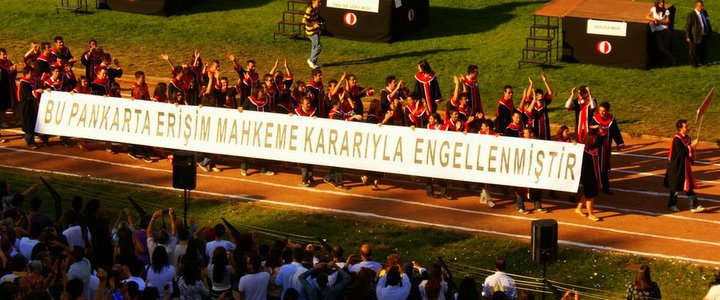
\includegraphics[width=0.8\textwidth]{project_graphics/banner1.jpg}
      \caption{Banner}
      \label{fig:Banner_1}
  \end{figure}
\begin{itemize}
\item \textbf{Puzzle.} Because it is cut out from very big and long banner (which is carried at graduation ceremony at METU, 2011). Every piece was a part of bigger banner. At that time there are serious debates about freedom on the internet. Most of the website are banned from the decision to the courts and they were not accessible. (Access to this banner is blocked by a court decision.) In Middle East Technical University there is a tradition that in graduation ceremony people walk through in the stadium and greet to the tribunes. With this event they carry some banners to express their feelings and criticize some realities in the country. This one of them. It is carried by students (new grads of Computer Engineering) The slogan decided by among the students and before the ceremony I printed out the slogan to carried out as many people as it can and easy to readable from the people who seat at the tribunes. After the ceremony I could not throw away this banner. I do not know what to do it, it is very big actually to store but I could not. I think that I will figure out later. Maybe I can use it as a draft paper. But is it worth to cut out this all long banner etc. Also to strengthen the banner and to prevent to tear while carried by the many people we are tape it from its boundaries. In other words some of the areas can not appropriate for writing. When I decided to this topic I remembered to this banner. It is stands in a corner in a dusty way. Now it is time use it. It waited very log time and it is time to revive again. Currently In turkey the problem of banning web-sites continues. Event it can said that people do not surprises when a website is blocked by the courts. It can be turn be a paper that people can freely express their ideas and feeling onto the it. Cut out them to the smaller pieces and make them as notebooks. They are part of puzzle. for the smaller parts what is written on them can not easily understandable. To realize what is the message is you have to bring together all of them again. But It is not possible, therefore website is a very good solution for them. All pages have unique patterns. Remaining parts of letter and tape. It provides unique layout for writing and I strongly think that all the notebooks after used have strong visual impact. 
\item \textbf{12:00 pm.} Burger King pockets from office where I work. Because it is launch time. It is collected at the same time.
\item \textbf{08:00 am.} Breakfast time. I think that these packages are used at the morning, very the beginning of the day.
\item \textbf{Friday Night.} (Maybe there can be another option related with traveling, or union). These notebook's pages are collected from restaurant "Varuna Gezgin". We go there to meet some friends after long time. One of them is coming from Australia, the other one is coming from Norway. they are my friends from the university. We united again at varuna gezgin. The place also interesting story. It is a place of travelers. It supports them. and the decoration of that place contains a lot of items collected from different sides of the world. The concept of the place and our meeting perfectly matched. I'm collecting the paper that are under the plates. When we are leaving this place, I ask the guy at the desk, I am making small notebooks and is it possible to exhibit there. I said that is it possible to give them to people. Firstly he asked me that selling them but I said no they are free and part of my thesis project. and later he offered me there are a lot of unused papers. I can give you. they are not used and waiting to be recycling. I took some of the papers, and that papers are part the sheets of these papers. 
% Name of the paper can be related with this place and related with the meaning. 
\item \textbf{Modsifters.} 
% Again I need some memory from here. 
% They are all my memories actually and I also turn my memories something different. Changing and constructing memories. And also others' memories... These project also contains others memories.

% Ersan hoca's packages. Elgins' papers etc. I do not know actually their stories. Maybe I can dream up stories for them. Creating histories from some of the trashes. They do not have proper memory with me, but I tried to construct memories, (fake memories can be said that.)

% Refer to 9 canlı. Never dies, revives again and again. Because trash moves in the community, even if thrown away can be find another use.

\end{itemize}

\subsubsection{Collected materials}
There are different papers and objects are used to produce papers
\begin{itemize}
\item Burger King packages, from office at launch time
\item Starbucks packages, from supervisor, office and my friend. Especially my supervisor and friend collect them from their friends and their own uses. They save them for me and later I take them later. 
\item Modshifters papers, that are covered on table and at the end of the day they are cut out and throw away. I go this place many times and every time questioned what they are doing to the papers. One of my visit we stay there at a late time and catch the garson collecting the old papers and prepearing tables to the next customer or day. I ask him to give me and he kindly accepted. From this paper I covered [x] notebooks. All of them contains track of people who sit down there. I do not know them and I am not sure that the paper that they are sit down turned to such a thing. 
\item Varuna Gezgin
\item Graduation banner
\item Tea bags.
% It is also realization of materials. Establishing different connection to them. Why is important? Identity construction.
\end{itemize}

\subsection{Website}
As I think that finding a place the discarded items is one of the main purposes of this project. As it finds a place peoples life again, it also finds another place in the digital space. ()

Mainly websites displays the story(History) of notebooks. Also it is a place to track the journey the notebooks. As I claimed that it is not a finished work. It does not completed transformation. It always continues. Therefore a website that anyone can reach share their progress via website. Anyone can later discover how they turned to new things etc. 

Collect peoples comment with this notebooks. As I leave notebooks different places I do not have connection with people who take them. This website also will help to collect/share peoples ideas about the notebooks.

It will contains a section for how notebooks are produced and the story behind it. The purpose is to record the creative process and share with the others. Revealing the process is significant to demystifiying the truth about the project. It makes it more clear that the object used here is actually transformed from something else. 

\textbf{Why website?} Maybe you can think that there are different methods to accomplish recording and sharing the process. In a gallery on a single table or a room it can be succeed. However it like the idea that website can evolve by time as this work evolve in time. I think it matches perfectly. This is not a finished work, it continues and so the website also. 

% Meaning of stories behind the process
There are different stories behind the objects. I try to record their stories (by photography and taking notes) but some of them were not possible. However I still use them in the work because even if I missed their story, with their materiality reveals their history. It still has a history but needs to rewritten. Maybe forgetting all the history maybe creates different notebook.

It is also co-authored work. Because many people helped me to collect the papers and also many people leave their trail to the paper and also they bring meaning to the them. After production of papers I also want them to continue as co-authored process. In other words many people will be part of this project. As people see different things on objects and bring them to me. the variety of things is increased in time. Because people sad me that \quotes{I thought that you can use it. Do you collect also these?}. After that time I want to continue as so. 

% I add the screenshoots of website. Also the development of it. Sketches of website. Navigation of it. User interaction. Use cases and actions. Functionalities.

% Documenting the progress. 

% It was not only that such characteristic was clearly suited for the exploration of human spaces such as home, but it was also that I am comfortably and confidently fluent in practicing photography

% Counter Argument:
% People may think and raise the question that none of notebooks is actually my work they belongs to others, others(Starbucks, Burger King) designed it and I am stealing their work. Here there are available different answers to the question. Firstly they are different once they are designed. Turned to different thing. I suggest that them to consider in different context like Duchamp. 

% I resurrect things that have been killed off... My work is all about the potential of materials — even when it looks like they've lost all possibilities. (Cornelia Parker) https://en.wikipedia.org/wiki/Cornelia_Parker

% These all memories and collected materials related with the my history. So why is it important for the other people. What can they found my memories. This is not theirs. How other people connect to the topic. They important for me but also I need to find something important for the other people. For example modshifter and varuna gezgin is one of them. This not only my experience. Some kind of shared memories and histories. What will find people in these notebooks.


%****************************************
% EXHIBITION
% Where people access them? How to design the experience here. The relationship with the location? 
% Pizza box, with l shape box. I need to find a place to put them. 
%
%........................................


%****************************************
%% Move to the other sections:
%
% Mandy Barker is an international award winning photographer whose work involving marine plastic debris has received global recognition. The motivation for her work is to raise awareness about plastic pollution in the world's oceans whilst highlighting the harmful affect on marine life and ultimately ourselves.
%........................................


%****************************************
% TODO Find a solution for this problem:
% Bu işin olması için ben insanlardan bir şeyler yapmalarını istiyorum. Yani aslında kendimde yapabilirim ama neden insanları da dahil ediyorum? Buradaki en önemli amaç değiştirmek dönüştürmek, sadece çöpü dönüştürmek yetmez, insanların fikirlerini de deönüştürmek gerekmek. ve bu bir süreç işi (şart mı tek bir yöntem bu mu?) İnsanlar nasıl değişir diye sormak gerekir o zaman. İnsanların değiştiğini dönüştüğünü gerçekten nasıl ölçeceğim ki? 

% important question: herkes neye ihtiyacı var ise onu toplar. ben neden niçin topluyorum. toplama sebepleri. dönüştürme sebepleri. neden sadece toplamakla yetinmiyorum. yani toplamak ile ayrıldığı noktalar nelerdir. Ben bir mana mı arıyorum? Yoksa kaybetmekten mi korkuyorum? Yeni kompozisyonlar oluşturmak istiyorum. Farklı karşımlar elde etmek istiyorum. Bir tür şaşırtmak durumu... Beklenmeyeni yapmak... En olmadık malzeme çöple çalışmak bu yüzden önemli benim için. 

%
% PROBLEM:
% In theoratical part I am focusing on actually the trash. But should I focus on paper trash? Is there any difference? Ya da ben oradaki bir farklılıktan besleniyor muyum? It is not totally paper, actually they are package. Examples can be given related with package material. It has a very short life. Not short actually. 

% How to establish the relationship between the collaboration and the trash? transforming them with the help of people. However, main discussion is not about collaboration. Here collaboration is a method to reach the aim of the project. In other words it is a methodology. There are different methodologies applied by artist to transform them. My methodology is to collaborate with the other people. My aim is to transform trash with people. Also make them to engage with trash. Trash is only one of the things discarded by the society. What is the importance of co-authored work?
%........................................


%****************************************
% Explain your project that I am like and child: 
% Collecting things means actually searching things. I'm searching for materials and also 
% What is the main focus in my work? Participation? Transformation? Composite of them? Trash? What else? 
%........................................

